\subsection{Reproducability}
All benchmarks were performed on an Intel Xeon E5 2697 processor with 64GB Ram, with Ubuntu 16.04 LTS, kernel 4.4.0 as operating system.
CSRM is implemented using Python3, the test system uses Python 3.5. 
The experiments use a fixed seed in order to guarantee determinism. Where relevant the configuration is given. 
An open source \href{https://bitbucket.org/bcardoen/csrm}{repository} holds the project's source code, benchmark scripts, analysis code and plots. The project dependencies are minimal making the project portable across any system that has a working Python3 implementation and pip as an installation manager. In order to run distributed the project requires an MPI implementation, which is available for most platforms.
\subsection{Benchmark problems}
Recent work on the convergence of GP-based SR \cite{SRAccur, SRBaseline} featured a set of benchmark problems that pose convergence problems for SR implementations. 
These 15 problems use at most five features, and are non linear arithmetic expressions using the standard set of base functions : (sin, cos, tan(h), log,$a^x$, /, *, modulo, abs, min, max, +, -).
 CSRM does not know which features are used, making the problem harder. In other words it assumes each problem is a function of 5 features which may or may not influence the expected outcome. This is an extra test in robustness for the algorithm, while also testing the algorithm's capability as a classifier. 
%\[
%1.57 + (24.3*x_3)\]
%\[0.23+14.2*\frac{x_3+x_1}{3.0*x_4}
%\]
%\[
%-5.41 + 4.9* ( \frac{x_3-x_0 +  \frac{x_1}{x_4} } {3*x_4} )
%\] 
%\[-2.3 + 0.13*\sin(x_2)\]
%\[3.0 + (2.13 * ln(x_4))\]
%\[1.3 + 0.13* \sqrt{x_0}\]
%\[213.80940889 - 213.80940889*e^{-0.54723748542*x_0}\]
%\[6.87+11*\sqrt{7.23*x_0*x_3*x_4}\]
%\[\frac{\sqrt{x_0}}{\ln(x_1)} *\frac{e^{x_2}}{x_3 ^ 2}\]
%\[ 0.81 + 24.3 * \frac{ 2.0*x_1+3.0*x_2^2} {4.0*x_3^3 + 5.0*x_4^4}\]
%\[6.87+ 11* \cos(7.23*x_0^3)\]
%\[2.0 - 2.1 * \cos(9.8*x_0) * \sin(1.3*x_4)\]
%\[32-3.0*  \frac{\tan(x_0)}{\tan(x_1)} *  \frac{tan(x_2)} {\tan(x_3)} \]
%\[22 - 4.2*((\cos(x_0)-\tan(x_1))*\frac{\tanh(x_2)}{\sin(x_3)}\]
%\[12.0 - 6.0* \frac{\tan(x_0)}{e^{x_1}} * (\ln(x_2)-\tan(x_3) ) \]
%                    


\subsection{Experiment setup}
Each process has a population of 20, initial depth of 4, max depth of 8, executes 20 phases of 20 generations each, with an archivesize of 20. Per phase the 4 best expressions are archived, the spreading policy distributes the best expressions over the communication links. The benchmark functions have at most 5 features, each with 20 sample points in the range [1,5]. The Grid and Tree topology will have single expression per link, the Random topology will have 2 per link. 25 processes are used, resulting in respectively 400, 15 ,50 being sent per phase. The random topology in this case contains 2 cliques of cycles.

%\begin{figure}
%    \centering
%    \begin{subfigure}{0.5\textwidth}
%    \centering
%        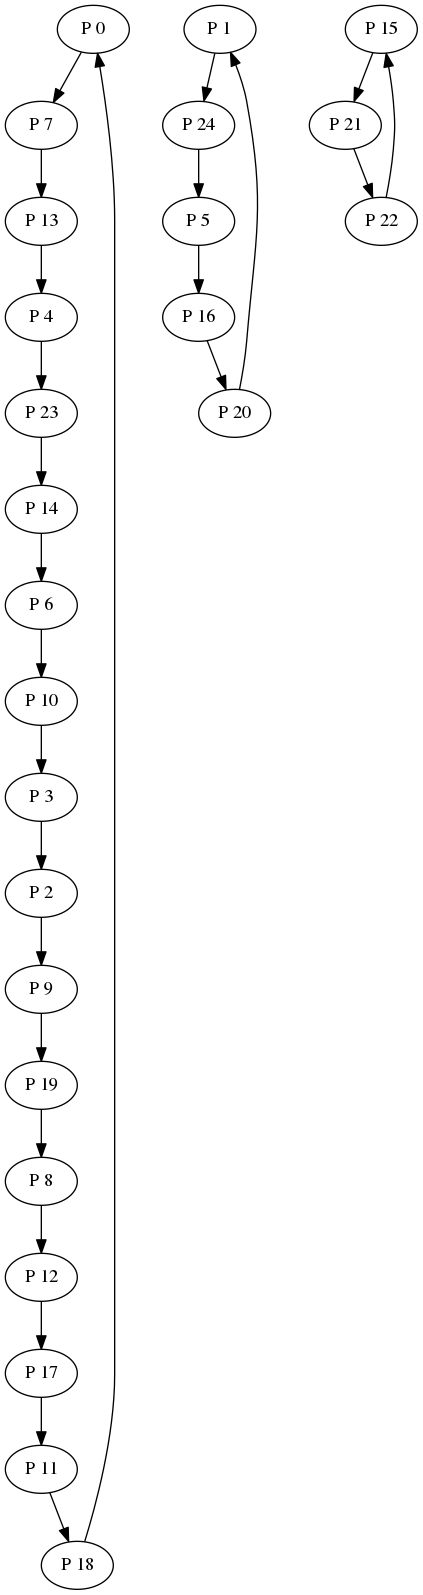
\includegraphics[width=0.5\linewidth]{figures/random25.png}
%        \caption{Random topology for 25 processes with one outgoing link per process.}
%    \end{subfigure}%
%    \begin{subfigure}{0.5\textwidth}
%    \centering
%        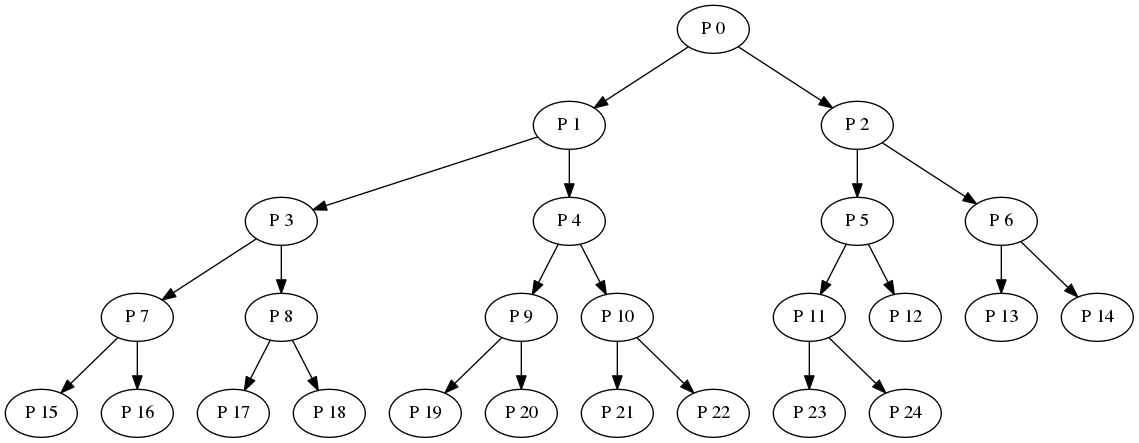
\includegraphics[width=0.5\linewidth]{figures/tree25.png}
%        \caption{Tree topology for 25 processes.}
%    \end{subfigure}
%    \caption{Tree and random topologies used in the experiment.}
%    \label{fig:experimenttopos}
%    \end{figure}

\subsubsection{Measures}
When the experiment ends the best 20 expressions from all processes are collected and scored. We measure best fitness on the training data, and best fitness on the validated data. 
Finally we record the mean fitness values of the best 5 expressions, both on the training and validation data. The mean is restricted to the upper quarter of the population specifically to measure how the best expressions are distributed. This measure records the convergence more accurately as the fittest expressions drive the convergence rate. 
\paragraph{Calculation}
The fitness values fluctuate strongly between the test problems and even between topologies. We apply a negative logarithmic scale :
$
f_t = -\log_{10}(f)
$
where f is either the best fitness value or the mean. Then we scale the results relative to the values obtained for the tree topology in order to measure relative gain or loss in orders of magnitude.
\subsubsection{Results}
\paragraph{Convergence}
\begin{figure}
    \centering
    \begin{subfigure}{0.6\textwidth}
    \centering
        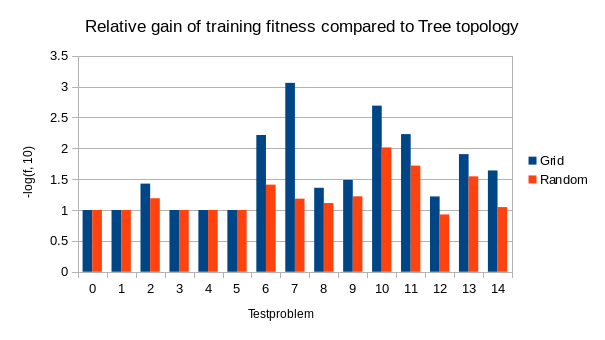
\includegraphics[width=0.8\linewidth]{figures/distributedbesttraining.png}
        \caption{Relative gain in best fitness of training data}
    \end{subfigure}%
    \begin{subfigure}{0.6\textwidth}
    \centering
        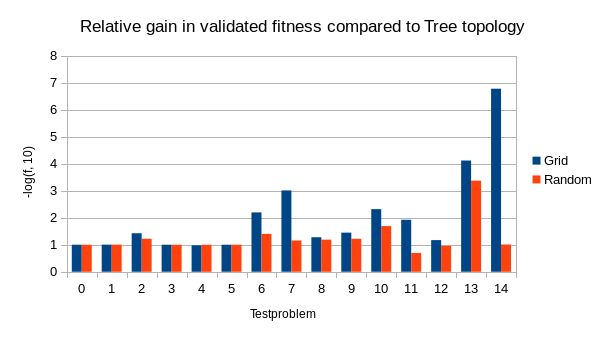
\includegraphics[width=0.8\linewidth]{figures/distributedbestvalidated.png}
        \caption{Relative gain in best fitness on full data.}
    \end{subfigure}
        \begin{subfigure}{0.6\textwidth}
    \centering
        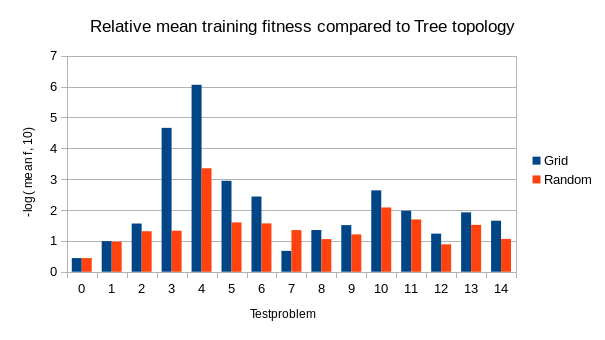
\includegraphics[width=0.8\linewidth]{figures/distributedmeantraining.png}
        \caption{Relative gain in mean fitness on training data.}
    \end{subfigure}%
    \begin{subfigure}{0.6\textwidth}
    \centering
        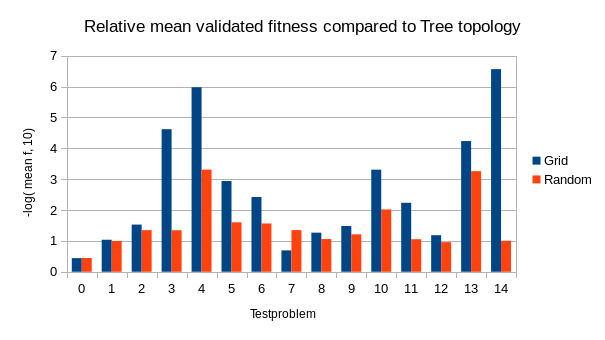
\includegraphics[width=0.8\linewidth]{figures/distributedmeanvalidated.png}
        \caption{Relative gain in mean fitness on full data.}
    \end{subfigure}
    \caption{Convergence differences between topologies.}
    \label{fig:distributedresults}
    \end{figure}
In Figure \ref{fig:distributedresults} we see how the topology affects convergence. The first observation we make is that the first 5 testproblems, with exception of the second, all have identical values for best fitness on training and validation data. The processes converged to zero fitness values for these problems, hence the identical results. 
The training fitness results in Figure \ref{fig:distributedresults}a indicate that the grid and random topology have superior convergence characteristics compared to the tree topology, with grid outperforming random on several testproblems. When we look at the fitness values on the validation data in Figure \ref{fig:distributedresults}b we see a more nuanced result. The grid topology is overall still the best choice, but the random topology has worse results for problems 11 and 12.
Next we look at the mean fitness values on training and validation data. Interestingly enough for problem 0 both random and grid score far worse than the tree topology. Overall the grid topology is still better for most problems, with the exception of problem 7. Note the similarity in pattern in the results here between training and validation data indicating that the predictive capability of the results is still good. If overfitting would have taken place we would see a reverse pattern in the results for the validation data.



\subparagraph{Measuring Overhead}
Cycles in the topology will lead to excessive synchronization and even serialization.
We measure the mean execution time for testproblem 6. The convergence characteristics using the three topologies differed significantly making this a good testcase. The processes will communicate 25 times. If the runtime of a single phase is too long, the overhead of communication will become hard to measure. If it is too short the overhead dominates the entire runtime. This second case is one we should try to avoid, it will unfairly penalize topologies with cycles forcing them to serialize. The runtime of a phase is dependent on the generations, population and depth ranges of the expressions. Ideally we would like for a practitioner to choose these parameters based on the problem at hand and not be constrained by synchronization considerations.
We compare the three topologies and use the disconnected or 'none' topology as a reference point, which has zero synchronization overhead.
This last topology has an ideal speedup of n, where n is the processcount, compared to a sequential process. From the synchronization overhead we can then derive the speedup each of the topologies is able to offer. In practice even the 'none' topology will have some synchronization overhead, as the root process has to collect all results from the other processes.
\begin{figure}
    \centering
    \begin{subfigure}{0.6\textwidth}
    \centering
        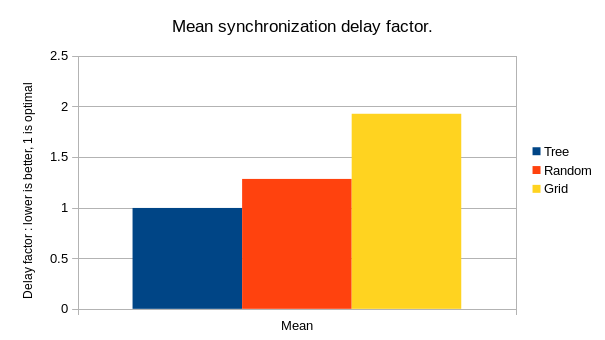
\includegraphics[width=0.8\linewidth]{figures/distributeddelaymean.png}
        \caption{Mean synchronization delay factor.}
    \end{subfigure}%
    \begin{subfigure}{0.6\textwidth}
    \centering
        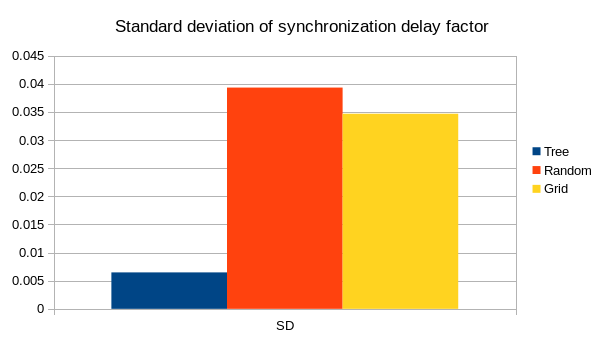
\includegraphics[width=0.8\linewidth]{figures/distributeddelaysd.png}
        \caption{Standard deviation of synchronization delay factor.}
    \end{subfigure}
    \caption{Synchronization overhead introduced by topologies.}
    \label{fig:distributeddelayresults}
    \end{figure}
In Figure \ref{fig:distributeddelayresults} we see that the tree topology has a near zero delay introduced by the synchronization. This is due to the delay tolerance we have built in in our implementation. The random topology has a mean delay factor of 1.3, the grid topology scores worst with a mean delay factor of nearly 2. This is easily translated in terms of speedup. A tree topology will have near linear speedup, a grid will have a speedup roughly half of that value and a random topology will have a speedup bracketed between those two. The standard deviation for the tree topology is significantly smaller indicating that a tree topology will have a far more predictable speedup.
